% defer/rcuusage.tex

\subsection{RCU Usage}
\label{sec:defer:RCU Usage}
\OriginallyPublished{Section}{sec:defer:RCU Usage}{RCU Usage}{Linux Weekly News}{PaulEMcKenney2008WhatIsRCUUsage}

\begin{table}[tb]
\begin{center}
\scriptsize
\begin{tabular}{l|l}
Mechanism RCU Replaces & Section \\
\hline
\hline
Reader-writer locking &
	Section~\ref{sec:defer:RCU is a Reader-Writer Lock Replacement} \\
Restricted reference-counting mechanism &
	Section~\ref{sec:defer:RCU is a Restricted Reference-Counting Mechanism} \\
Bulk reference-counting mechanism &
	Section~\ref{sec:defer:RCU is a Bulk Reference-Counting Mechanism} \\
Poor man's garbage collector &
	Section~\ref{sec:defer:RCU is a Poor Man's Garbage Collector} \\
Existence Guarantees &
	Section~\ref{sec:defer:RCU is a Way of Providing Existence Guarantees} \\
Type-Safe Memory &
	Section~\ref{sec:deferRCU is a Way of Providing Type-Safe Memory} \\
Wait for things to finish &
	Section~\ref{sec:deferRCU is a Way of Waiting for Things to Finish} \\
\end{tabular}
\end{center}
\caption{RCU Usage}
\label{tab:defer:RCU Usage}
\end{table}

This section answers the question "what is RCU?" from the viewpoint
of the uses to which RCU can be put.
Because RCU is most frequently used to replace some existing mechanism,
we look at it primarily in terms of its relationship to such mechanisms,
as listed in Table~\ref{tab:defer:RCU Usage}.
Following the sections listed in this table,
Section~\ref{sec:defer:RCU Usage Summary} provides a summary.

\subsubsection{RCU is a Reader-Writer Lock Replacement}
\label{sec:defer:RCU is a Reader-Writer Lock Replacement}

Perhaps the most common use of RCU within the Linux kernel is as
a replacement for reader-writer locking in read-intensive situations.
Nevertheless, this use of RCU was not immediately apparent to me
at the outset, in fact, I chose to implement something similar to
\url{brlock} before implementing a general-purpose RCU implementation
back in the early 1990s.
Each and every one of the uses I envisioned for the proto-brlock
primitive was instead implemented using RCU.
In fact, it was more than
three years before the proto-\url{brlock} primitive saw its first use.
Boy, did I feel foolish!

The key similarity between RCU and reader-writer locking is that
both have read-side critical sections that can execute in parallel.
In fact, in some cases, it is possible to mechanically substitute RCU API
members for the corresponding reader-writer lock API members.
But first, why bother?

Advantages of RCU include performance,
deadlock immunity, and realtime latency.
There are, of course, limitations to RCU, including the fact that
readers and updaters run concurrently, that low-priority RCU readers
can block high-priority threads waiting for a grace period to elapse,
and that grace-period latencies can extend for many milliseconds.
These advantages and limitations are discussed in the following sections.

\paragraph{Performance}

\begin{figure}[tb]
\begin{center}
\resizebox{3in}{!}{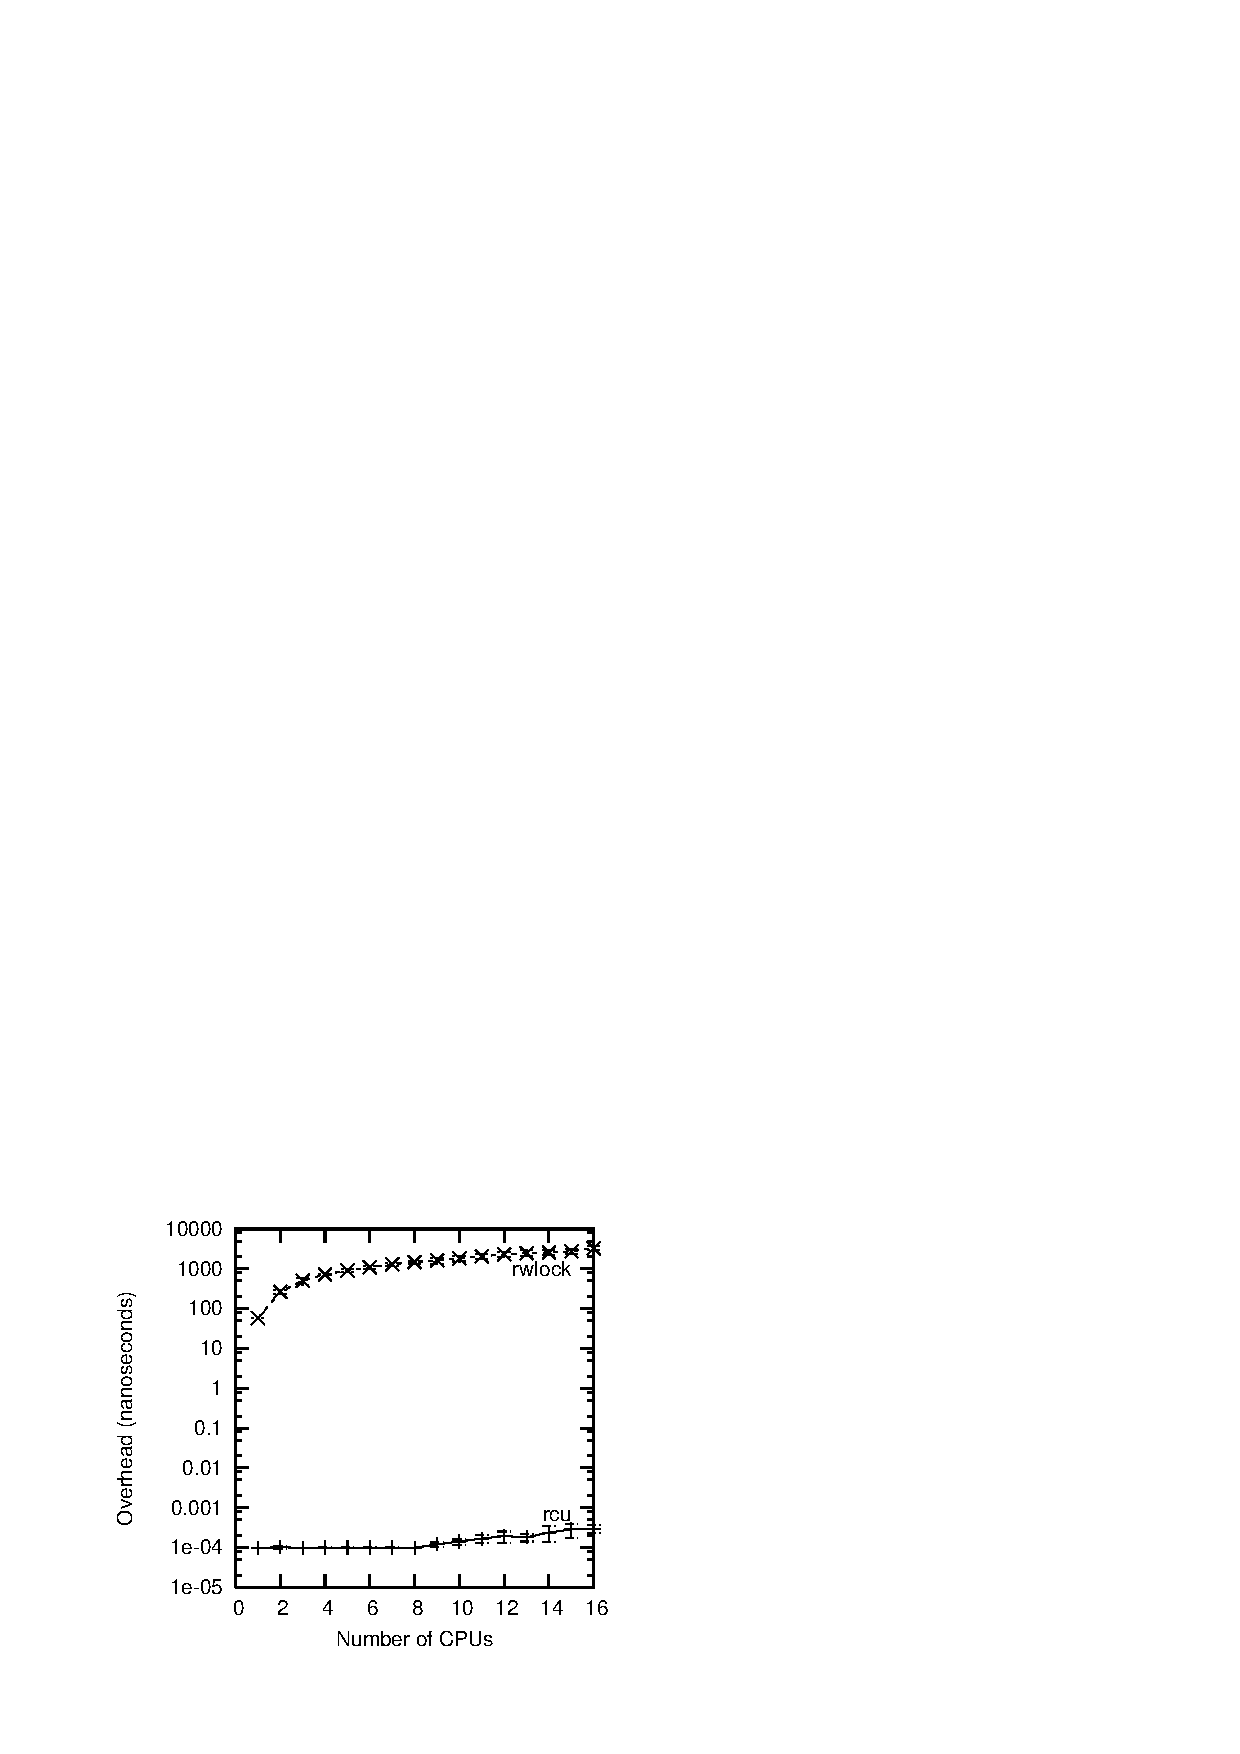
\includegraphics{defer/rwlockRCUperf}}
\end{center}
\caption{Performance Advantage of RCU Over Reader-Writer Locking}
\label{fig:defer:Performance Advantage of RCU Over Reader-Writer Locking}
\end{figure}

The read-side performance advantages of RCU over reader-writer locking
are shown in
Figure~\ref{fig:defer:Performance Advantage of RCU Over Reader-Writer Locking}.

\QuickQuiz{}
	WTF???
	How the heck do you expect me to believe that RCU has a
	100-femtosecond overhead when the clock period at 3GHz is more than
	300 \emph{picoseconds}?
\QuickQuizAnswer{
	First, consider that the inner loop used to
	take this measurement is as follows:

\vspace{5pt}
\begin{minipage}[t]{\columnwidth}
\small
\begin{verbatim}
  1 for (i = 0; i < CSCOUNT_SCALE; i++) {
  2   rcu_read_lock();
  3   rcu_read_unlock();
  4 }
\end{verbatim}
\end{minipage}
\vspace{5pt}

	Next, consider the effective definitions of \url{rcu_read_lock()}
	and \url{rcu_read_unlock()}:

\vspace{5pt}
\begin{minipage}[t]{\columnwidth}
\small
\begin{verbatim}
  1 #define rcu_read_lock()   do { } while (0)
  2 #define rcu_read_unlock() do { } while (0)
\end{verbatim}
\end{minipage}
\vspace{5pt}

	Consider also that the compiler does simple optimizations,
	allowing it to replace the loop with:

\vspace{5pt}
\begin{minipage}[t]{\columnwidth}
\small
\begin{verbatim}
i = CSCOUNT_SCALE;
\end{verbatim}
\end{minipage}
\vspace{5pt}

	So the "measurement" of 100 femtoseconds is simply the fixed
	overhead of the timing measurements divided by the number of
	passes through the inner loop containing the calls
	to \url{rcu_read_lock()} and \url{rcu_read_unlock()}.
	And therefore, this measurement really is in error, in fact,
	in error by an arbitrary number of orders of magnitude.
	As you can see by the definition of \url{rcu_read_lock()}
	and \url{rcu_read_unlock()} above, the actual overhead
	is precisely zero.

	It certainly is not every day that a timing measurement of
	100 femtoseconds turns out to be an overestimate!
} \QuickQuizEnd

Note that reader-writer locking is orders of magnitude slower than RCU
on a single CPU, and is almost two \emph{additional} orders of magnitude
slower on 16 CPUs.
In contrast, RCU scales quite well.
In both cases, the error bars span a single standard deviation in either
direction.

\begin{figure}[tb]
\begin{center}
\resizebox{3in}{!}{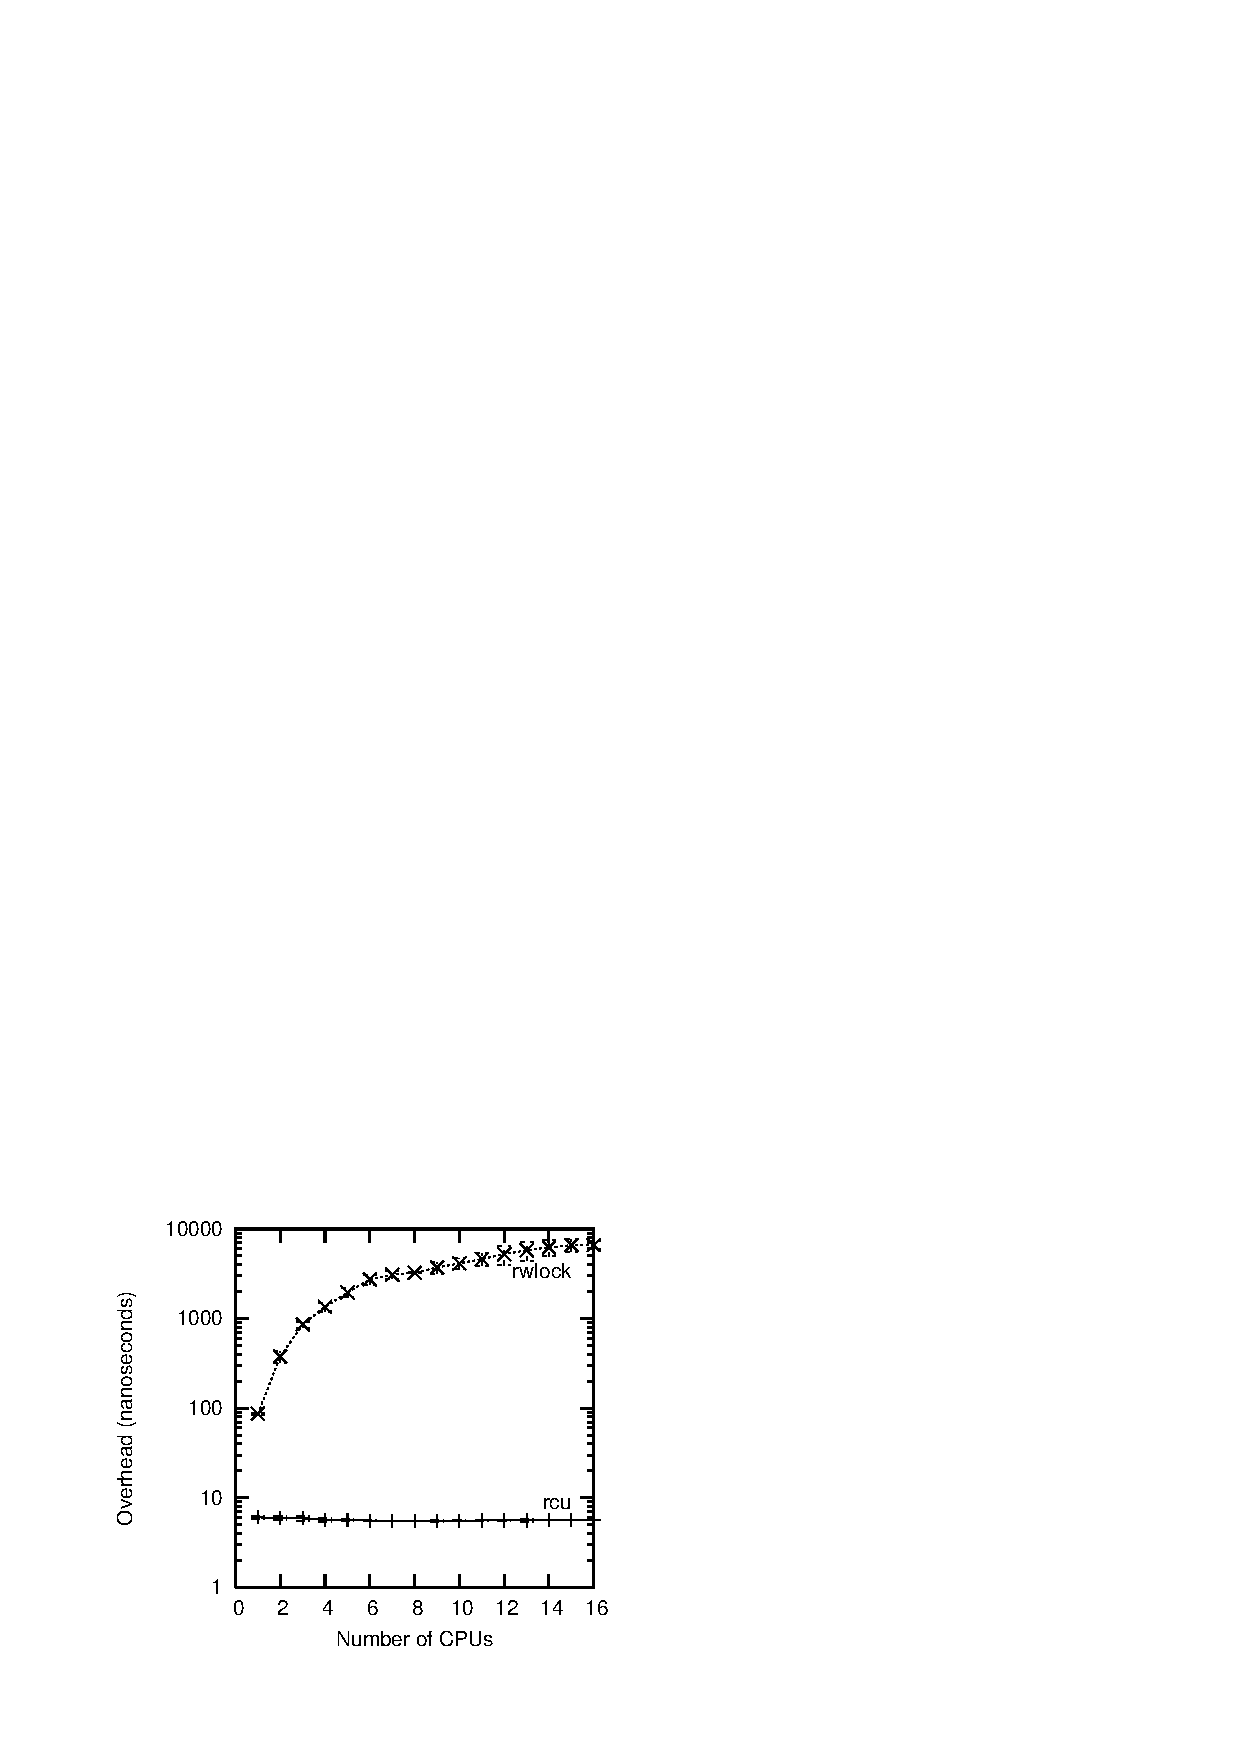
\includegraphics{defer/rwlockRCUperfPREEMPT}}
\end{center}
\caption{Performance Advantage of Preemptible RCU Over Reader-Writer Locking}
\label{fig:defer:Performance Advantage of Preemptible RCU Over Reader-Writer Locking}
\end{figure}

A more moderate view may be obtained from a \url{CONFIG_PREEMPT}
kernel, though RCU still beats reader-writer locking by between one and
three orders of magnitude, as shown in
Figure~\ref{fig:defer:Performance Advantage of Preemptible RCU Over Reader-Writer Locking}.
Note the high variability of reader-writer locking at larger numbers of CPUs.
The error bars span a single standard deviation in either direction.

\begin{figure}[tb]
\begin{center}
\resizebox{3in}{!}{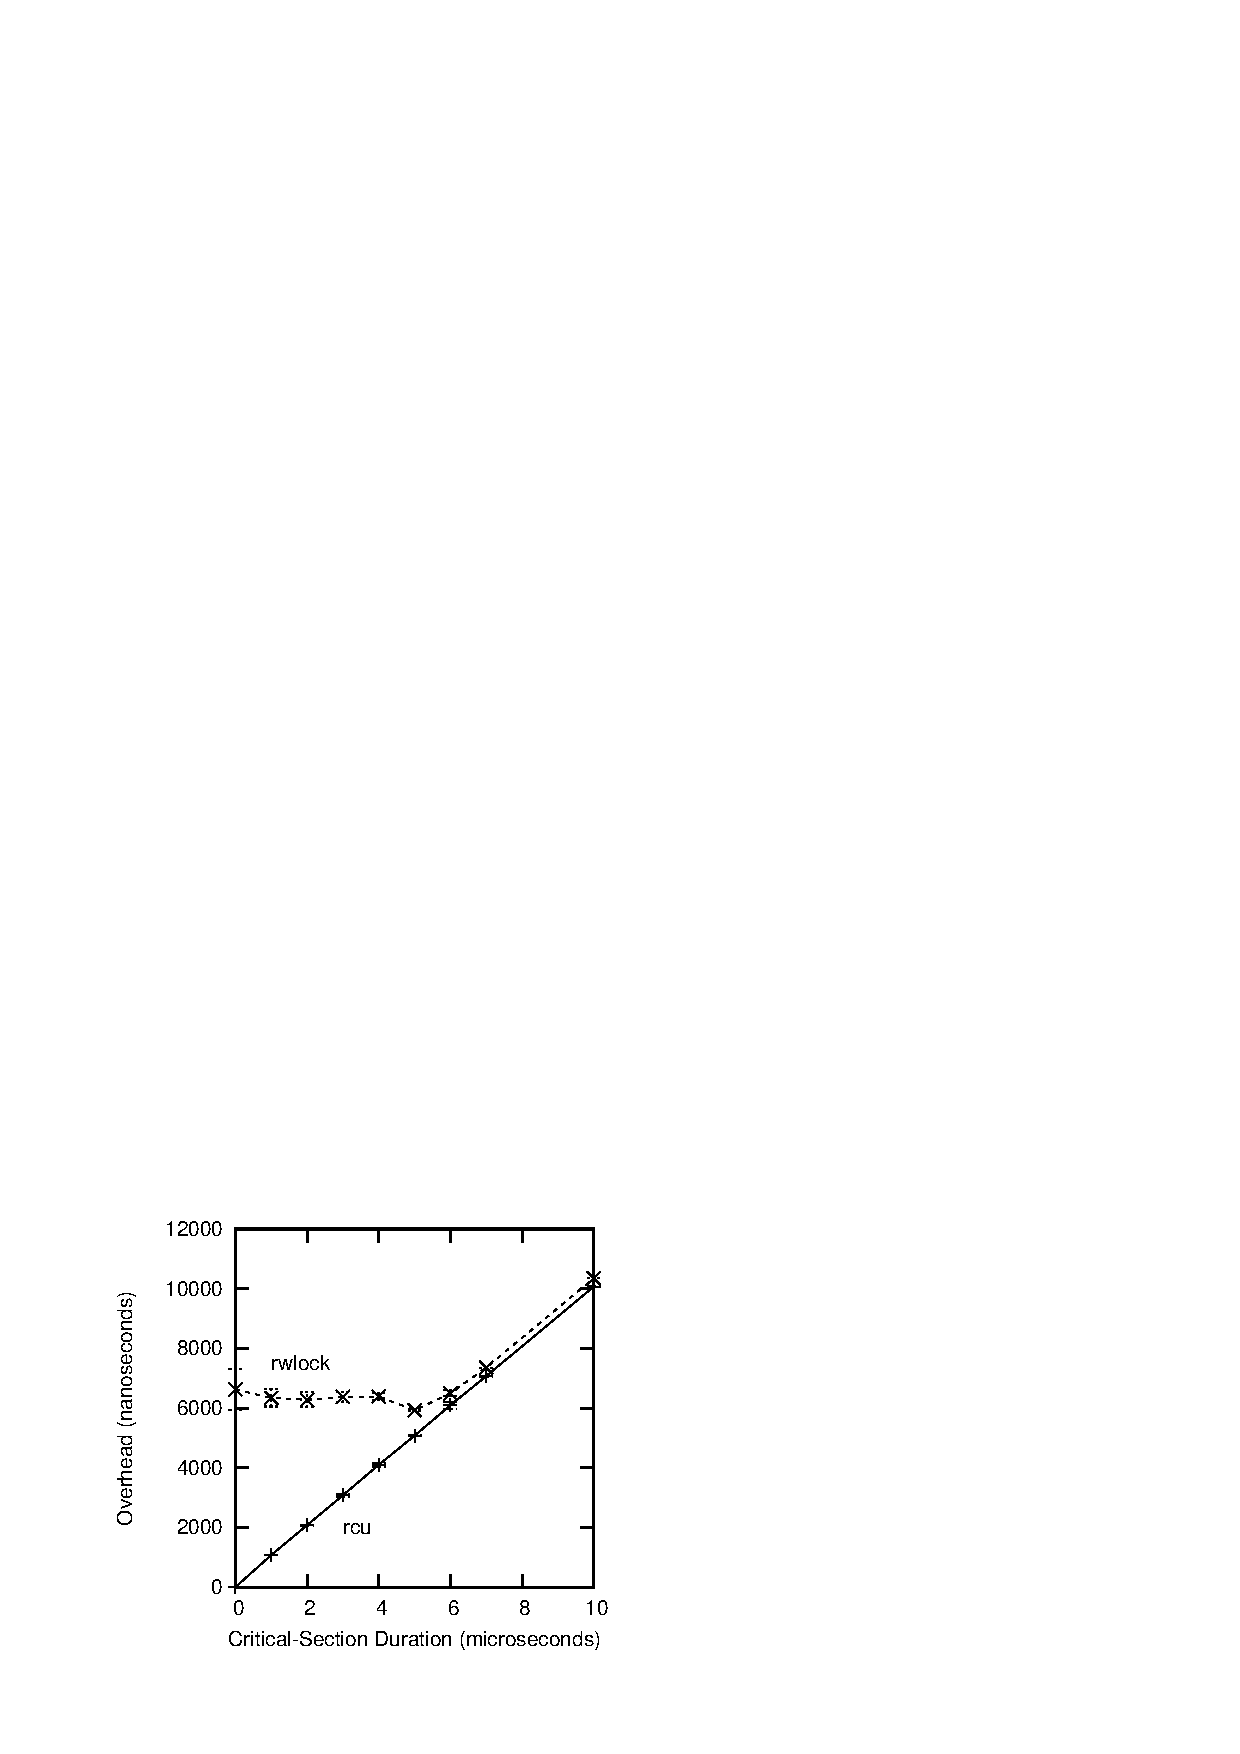
\includegraphics{defer/rwlockRCUperfwtPREEMPT}}
\end{center}
\caption{Comparison of RCU to Reader-Writer Locking as Function of Critical-Section Duration}
\label{fig:defer:Comparison of RCU to Reader-Writer Locking as Function of Critical-Section Duration}
\end{figure}

Of course, the low performance of reader-writer locking in
Figure~\ref{fig:defer:Performance Advantage of Preemptible RCU Over Reader-Writer Locking}
is exaggerated by the unrealistic zero-length critical sections.
The performance advantages of RCU become less significant as the overhead
of the critical section increases, as shown in
Figure~\ref{fig:defer:Comparison of RCU to Reader-Writer Locking as Function of Critical-Section Duration}
for a 16-CPU system,
in which the y-axis represents the sum of the overhead
of the read-side primitives and that of the critical section.

\QuickQuiz{}
	Why does both the variability and overhead of rwlock decrease as the
	critical-section overhead increases?
\QuickQuizAnswer{
	Because the contention on the underlying
	\url{rwlock_t} decreases as the critical-section overhead
	increases.
	However, the rwlock overhead will not quite drop to that on a single
	CPU because of cache-thrashing overhead.
} \QuickQuizEnd

However, this observation must be tempered by the fact that
a number of system calls (and thus any RCU read-side critical sections
that they contain) can complete within a few microseconds.

In addition, as is discussed in the next section,
RCU read-side primitives are almost entirely deadlock-immune.


\paragraph{Deadlock Immunity}

Although RCU offers significant performance advantages for
read-mostly workloads, one of the primary reasons for creating
RCU in the first place was in fact its immunity to read-side
deadlocks.
This immunity stems from the fact that
RCU read-side primitives do not block, spin, or even
do backwards branches, so that their execution time is deterministic.
It is therefore impossible for them to participate in a deadlock
cycle.

\QuickQuiz{}
	Is there an exception to this deadlock immunity, and if so,
	what sequence of events could lead to deadlock?
\QuickQuizAnswer{
	One way to cause a deadlock cycle involving
	RCU read-side primitives is via the following (illegal) sequence
	of statements:

\vspace{5pt}
\begin{minipage}[t]{\columnwidth}
\small
\begin{verbatim}
idx = srcu_read_lock(&srcucb);
synchronize_srcu(&srcucb);
srcu_read_unlock(&srcucb, idx);
\end{verbatim}
\end{minipage}
\vspace{5pt}

	The \url{synchronize_rcu()} cannot return until all
	pre-existing SRCU read-side critical sections complete, but
	is enclosed in an SRCU read-side critical section that cannot
	complete until the \url{synchronize_srcu()} returns.
	The result is a classic self-deadlock--you get the same
	effect when attempting to write-acquire a reader-writer lock
	while read-holding it.

	Note that this self-deadlock scenario does not apply to
	RCU Classic, because the context switch performed by the
	\url{synchronize_rcu()} would act as a quiescent state
	for this CPU, allowing a grace period to complete.
	However, this is if anything even worse, because data used
	by the RCU read-side critical section might be freed as a
	result of the grace period completing.

	In short, do not invoke synchronous RCU update-side primitives
	from within an RCU read-side critical section.
} \QuickQuizEnd

An interesting consequence of RCU's read-side deadlock immunity is
that it is possible to unconditionally upgrade an RCU
reader to an RCU updater.
Attempting to do such an upgrade with reader-writer locking results
in deadlock.
A sample code fragment that does an RCU read-to-update upgrade follows:

\vspace{5pt}
\begin{minipage}[t]{\columnwidth}
\scriptsize
\begin{verbatim}
  1 rcu_read_lock();
  2 list_for_each_entry_rcu(p, \&head, list_field) {
  3   do_something_with(p);
  4   if (need_update(p)) {
  5     spin_lock(\my_lock);
  6     do_update(p);
  7     spin_unlock(\&my_lock);
  8   }
  9 }
 10 rcu_read_unlock();
\end{verbatim}
\end{minipage}
\vspace{5pt}

Note that \url{do_update()} is executed under
the protection of the lock \emph{and} under RCU read-side protection.

Another interesting consequence of RCU's deadlock immunity is its
immunity to a large class of priority inversion problems.
For example, low-priority RCU readers cannot prevent a high-priority
RCU updater from acquiring the update-side lock.
Similarly, a low-priority RCU updater cannot prevent high-priority
RCU readers from entering an RCU read-side critical section.

\paragraph{Realtime Latency}

Because RCU read-side primitives neither spin nor block, they offer
excellent realtime latencies.
In addition, as noted earlier, this means that they are
immune to priority inversion
involving the RCU read-side primitives and locks.

However, RCU is susceptible to more subtle priority-inversion scenarios,
for example, a high-priority process blocked waiting for an RCU
grace period to elapse can be blocked by low-priority RCU readers
in -rt kernels.
This can be solved by using RCU priority
boosting~\cite{PaulEMcKenney2007BoostRCU,DinakarGuniguntala2008IBMSysJ}.

\paragraph{RCU Readers and Updaters Run Concurrently}

Because RCU readers never spin nor block, and because updaters are not
subject to any sort of rollback or abort semantics, RCU readers and
updaters must necessarily run concurrently.
This means that RCU readers might access stale data, and might even
see inconsistencies, either of which can render conversion from reader-writer
locking to RCU non-trivial.

\begin{figure}[tb]
\begin{center}
\resizebox{3in}{!}{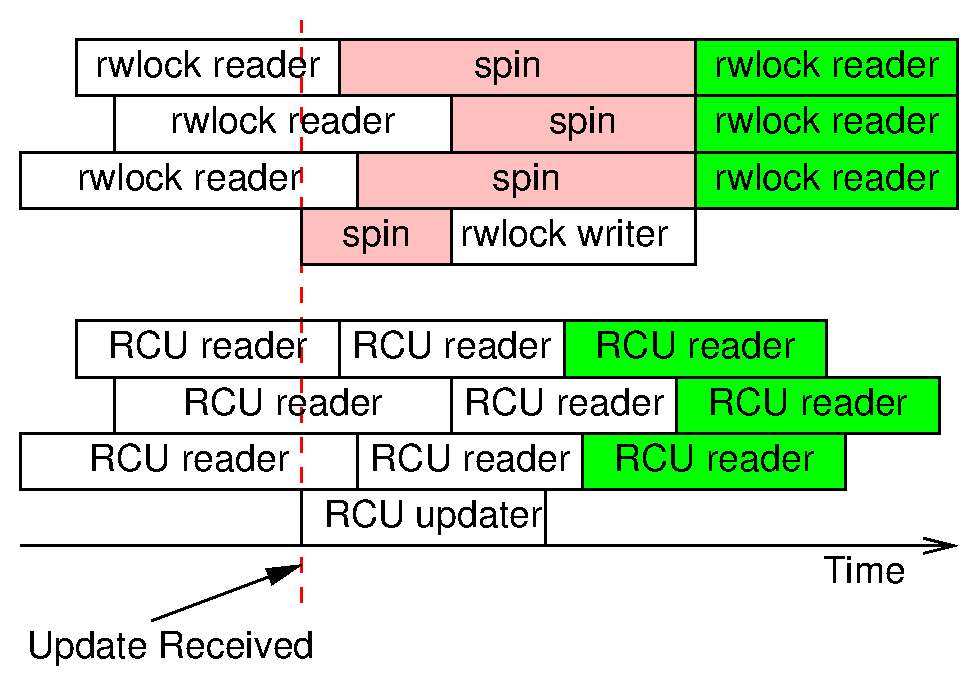
\includegraphics{defer/rwlockRCUupdate}}
\end{center}
\caption{Response Time of RCU vs. Reader-Writer Locking}
\label{fig:defer:Response Time of RCU vs. Reader-Writer Locking}
\end{figure}

However, in a surprisingly large number of situations, inconsistencies and
stale data are not problems.
The classic example is the networking routing table.
Because routing updates can take considerable time to reach a given
system (seconds or even minutes), the system will have been sending
packets the wrong way for quite some time when the update arrives.
It is usually not a problem to continue sending updates the wrong
way for a few additional milliseconds.
Furthermore, because RCU updaters can make changes without waiting for
RCU readers to finish,
the RCU readers might well see the change more quickly than would
batch-fair
reader-writer-locking readers, as shown in
Figure~\ref{fig:defer:Response Time of RCU vs. Reader-Writer Locking}.

Once the update is received, the rwlock writer cannot proceed until the
last reader completes, and subsequent readers cannot proceed until the
writer completes.
However, these subsequent readers are guaranteed to see the new value,
as indicated by the green background.
In contrast, RCU readers and updaters do not block each other, which permits
the RCU readers to see the updated values sooner.
Of course, because their execution overlaps that of the RCU updater,
\emph{all} of the RCU readers might well see updated values, including
the three readers that started before the update.
Nevertheless only the RCU readers with green backgrounds
are \emph{guaranteed} to see the updated values, again, as indicated
by the green background.

Reader-writer locking and RCU simply provide different guarantees.
With reader-writer locking, any reader that begins after the writer begins
is guaranteed to see new values, and any reader that attempts to
begin while the writer is spinning might or might not see new values,
depending on the reader/writer preference of the rwlock implementation in
question.
In contrast, with RCU, any reader that begins after the updater completes
is guaranteed to see new values, and any reader that completes after the
updater begins might or might not see new values, depending on timing.

The key point here is that, although reader-writer locking does
indeed guarantee consistency within the confines of the computer system,
there are situations where this consistency comes at the price of
increased \emph{inconsistency} with the outside world.
In other words, reader-writer locking obtains internal consistency at the
price of silently stale data with respect to the outside world.

Nevertheless, there are situations where inconsistency and stale
data within the confines of the system cannot be tolerated.
Fortunately,
there are a number of approaches that avoid inconsistency and stale
data~\cite{PaulEdwardMcKenneyPhD,Arcangeli03}, and some
methods based on reference counting are discussed in
Section~\ref{sec:defer:Reference Counting}.

\paragraph{Low-Priority RCU Readers Can Block High-Priority Reclaimers}

In Realtime RCU~\cite{DinakarGuniguntala2008IBMSysJ} (see
Section~\ref{app:rcuimpl:Preemptible RCU}),
SRCU~\cite{PaulEMcKenney2006c} (see
Section~\ref{app:rcuimpl:Sleepable RCU Implementation}, or
QRCU~\cite{PaulEMcKenney2007QRCUspin} (see
Section~\ref{app:formal:Promela Example: QRCU},
each of which is described in
the final installment of this series,
a preempted reader will prevent
a grace period from completing, even if a high-priority task is
blocked waiting for that grace period to complete.
Realtime RCU can avoid this problem by substituting \url{call_rcu()}
for \url{synchronize_rcu()} or by using RCU priority
boosting~\cite{PaulEMcKenney2007BoostRCU,DinakarGuniguntala2008IBMSysJ},
which is still in experimental status as of early 2008.
It might become necessary to augment SRCU and QRCU with priority boosting,
but not before a clear real-world need is demonstrated.

\paragraph{RCU Grace Periods Extend for Many Milliseconds}

With the exception of QRCU and several of the ``toy'' RCU implementations
described in
Section~\ref{defer:``Toy'' RCU Implementations},
RCU grace periods extend for multiple milliseconds.
Although there are a number of techniques to render such long delays
harmless, including use of the asynchronous interfaces where available
(\url{call_rcu()} and \url{call_rcu_bh()}), this situation
is a major reason for the rule of thumb that RCU be used in read-mostly
situations.

\paragraph{Comparison of Reader-Writer Locking and RCU Code}

In the best case, the conversion from reader-writer locking to RCU
is quite simple, as shown in
Figures~\ref{fig:defer:Converting Reader-Writer Locking to RCU: Data},
\ref{fig:defer:Converting Reader-Writer Locking to RCU: Search},
and
\ref{fig:defer:Converting Reader-Writer Locking to RCU: Deletion},
all taken from
Wikipedia~\cite{WikipediaRCU}.

\begin{figure*}[htbp]
{ \scriptsize \centering
\begin{verbatim}
 1 struct el {                           1 struct el {
 2   struct list_head lp;                2   struct list_head lp;
 3   long key;                           3   long key;
 4   spinlock_t mutex;                   4   spinlock_t mutex;
 5   int data;                           5   int data;
 6   /* Other data fields */             6   /* Other data fields */
 7 };                                    7 };
 8 DEFINE_RWLOCK(listmutex);             8 DEFINE_SPINLOCK(listmutex);
 9 LIST_HEAD(head);                      9 LIST_HEAD(head);
\end{verbatim}
}
\caption{Converting Reader-Writer Locking to RCU: Data}
\label{fig:defer:Converting Reader-Writer Locking to RCU: Data}
\end{figure*}

\begin{figure*}[htbp]
{ \scriptsize \centering
\begin{verbatim}
 1 int search(long key, int *result)     1 int search(long key, int *result)
 2 {                                     2 {
 3   struct el *p;                       3   struct el *p;
 4                                       4
 5   read_lock(&listmutex);              5   rcu_read_lock();
 6   list_for_each_entry(p, &head, lp) { 6   list_for_each_entry_rcu(p, &head, lp) {
 7     if (p->key == key) {              7     if (p->key == key) {
 8       *result = p->data;              8       *result = p->data;
 9       read_unlock(&listmutex);        9       rcu_read_unlock();
10       return 1;                      10       return 1;
11     }                                11     }
12   }                                  12   }
13   read_unlock(&listmutex);           13   rcu_read_unlock();
14   return 0;                          14   return 0;
15 }                                    15 }
\end{verbatim}
}
\caption{Converting Reader-Writer Locking to RCU: Search}
\label{fig:defer:Converting Reader-Writer Locking to RCU: Search}
\end{figure*}

\begin{figure*}[htbp]
{ \scriptsize \centering
\begin{verbatim}
 1 int delete(long key)                  1 int delete(long key)
 2 {                                     2 {
 3   struct el *p;                       3   struct el *p;
 4                                       4
 5   write_lock(&listmutex);             5   spin_lock(&listmutex);
 6   list_for_each_entry(p, &head, lp) { 6   list_for_each_entry(p, &head, lp) {
 7     if (p->key == key) {              7     if (p->key == key) {
 8       list_del(&p->lp);               8       list_del_rcu(&p->lp);
 9       write_unlock(&listmutex);       9       spin_unlock(&listmutex);
                                        10       synchronize_rcu();
10       kfree(p);                      11       kfree(p);
11       return 1;                      12       return 1;
12     }                                13     }
13   }                                  14   }
14   write_unlock(&listmutex);          15   spin_unlock(&listmutex);
15   return 0;                          16   return 0;
16 }                                    17 }
\end{verbatim}
}
\caption{Converting Reader-Writer Locking to RCU: Deletion}
\label{fig:defer:Converting Reader-Writer Locking to RCU: Deletion}
\end{figure*}

More-elaborate cases of replacing reader-writer locking with RCU
are beyond the scope of this document.

\subsubsection{RCU is a Restricted Reference-Counting Mechanism}
\label{sec:defer:RCU is a Restricted Reference-Counting Mechanism}

Because grace periods are not allowed to complete while
there is an RCU read-side critical section in progress,
the RCU read-side primitives may be used as a restricted
reference-counting mechanism.
For example, consider the following code fragment:

\vspace{5pt}
\begin{minipage}[t]{\columnwidth}
\scriptsize
\begin{verbatim}
  1 rcu_read_lock();  /* acquire reference. */
  2 p = rcu_dereference(head);
  3 /* do something with p. */
  4 rcu_read_unlock();  /* release reference. */
\end{verbatim}
\end{minipage}
\vspace{5pt}

The \url{rcu_read_lock()} primitive can be thought of as
acquiring a reference to \url{p}, because a grace period
starting after the \url{rcu_dereference()} assigns to \url{p}
cannot possibly end until after we reach the matching
\url{rcu_read_unlock()}.
This reference-counting scheme is restricted in that
we are not allowed to block in RCU read-side critical sections,
nor are we permitted to hand off an RCU read-side critical section
from one task to another.

Regardless of these restrictions,
the following code can safely delete \url{p}:

\vspace{5pt}
\begin{minipage}[t]{\columnwidth}
\scriptsize
\begin{verbatim}
  1 spin_lock(\&mylock);
  2 p = head;
  3 rcu_assign_pointer(head, NULL);
  4 spin_unlock(\&mylock);
  5 /* Wait for all references to be released. */
  6 synchronize_rcu();
  7 kfree(p);
\end{verbatim}
\end{minipage}
\vspace{5pt}

The assignment to \url{head} prevents any future references
to \url{p} from being acquired, and the \url{synchronize_rcu()}
waits for any previously acquired references to be released.

\QuickQuiz{}
	But wait!
	This is exactly the same code that might be used when thinking
	of RCU as a replacement for reader-writer locking!
	What gives?
\QuickQuizAnswer{
	This is an effect of the Law of Toy Examples:
	beyond a certain point, the code fragments look the same.
	The only difference is in how we think about the code.
	However, this difference can be extremely important.
	For but one example of the importance, consider that if we think
	of RCU as a restricted reference counting scheme, we would never
	be fooled into thinking that the updates would exclude the RCU
	read-side critical sections.

	It nevertheless is often useful to think of RCU as a replacement
	for reader-writer locking, for example, when you are replacing
	reader-writer locking with RCU.
} \QuickQuizEnd

Of course, RCU can also be combined with traditional reference counting,
as has been discussed on LKML and as summarized in
Section~\ref{sec:defer:Reference Counting}.

\begin{figure}[tb]
\begin{center}
\resizebox{3in}{!}{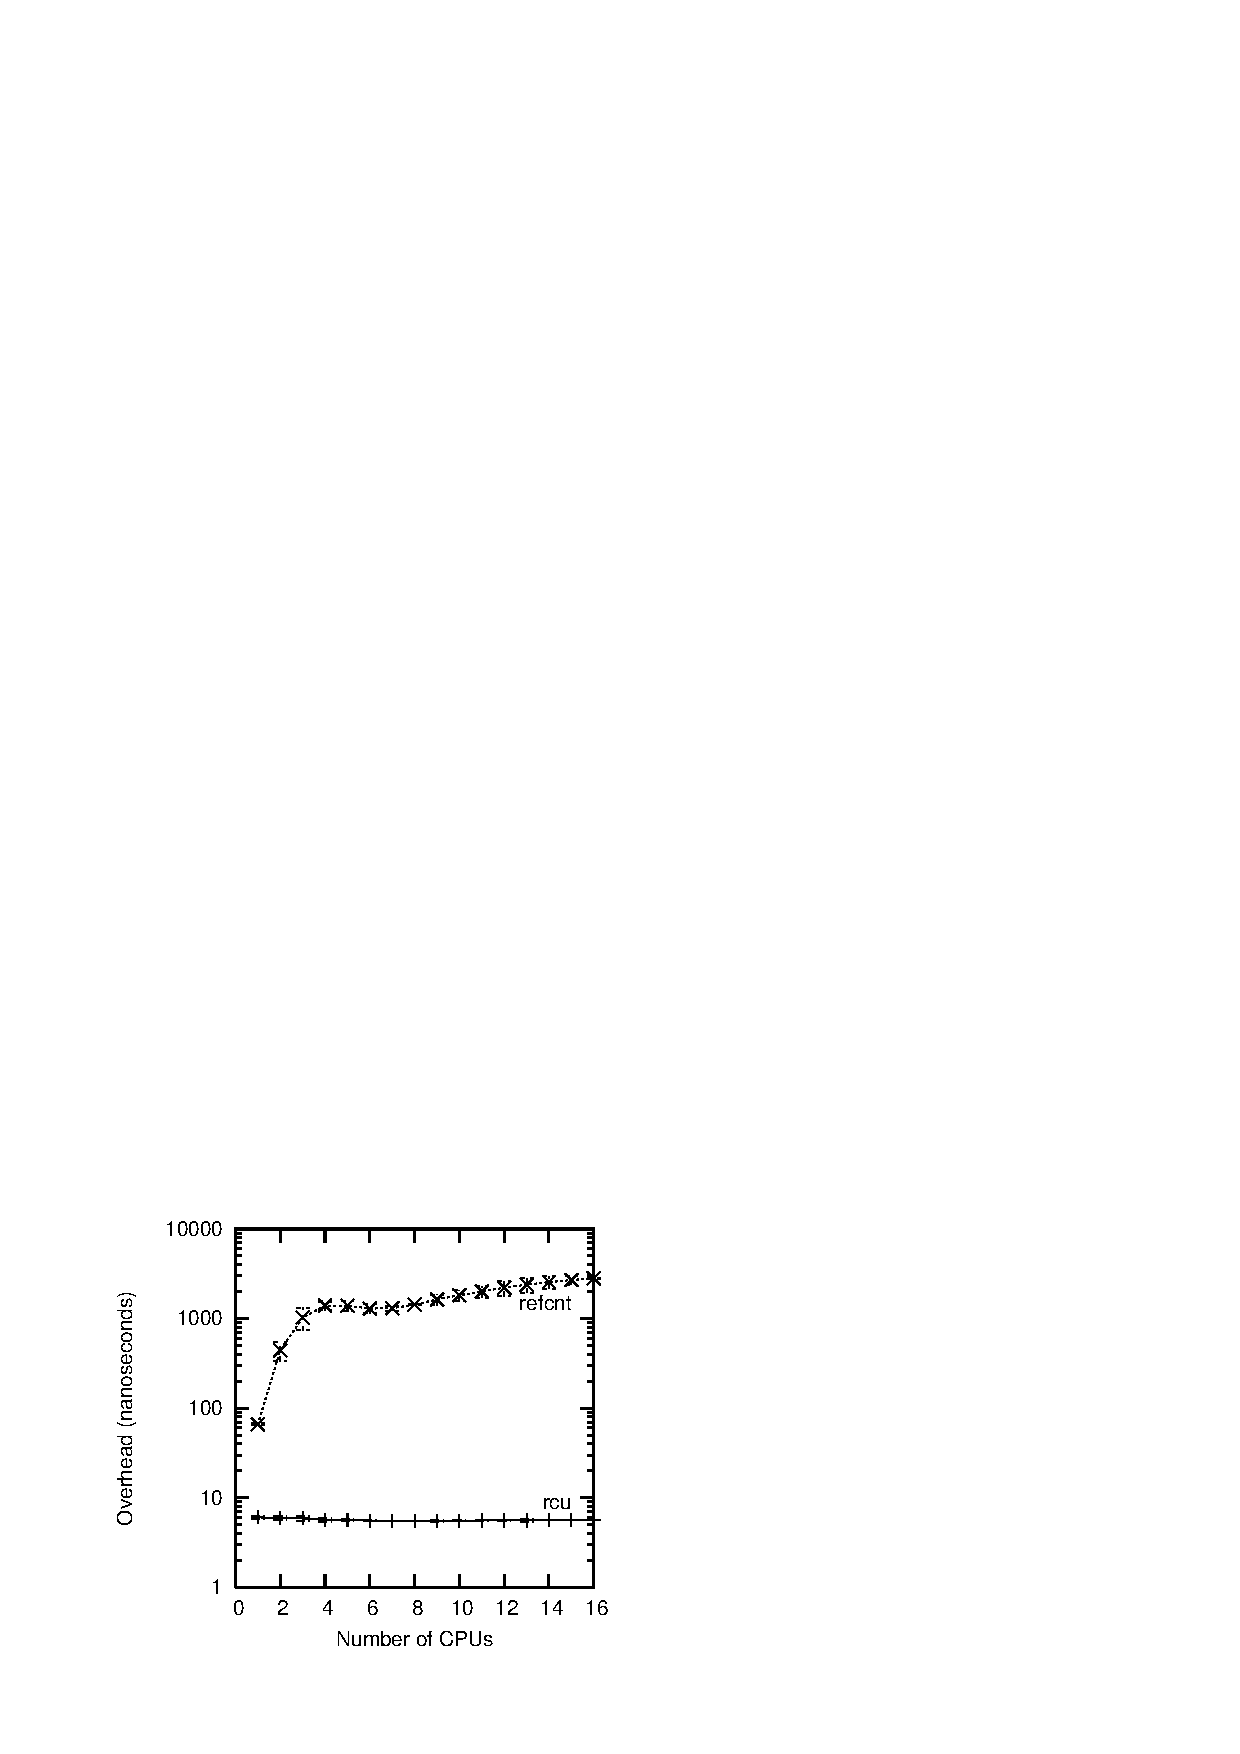
\includegraphics{defer/refRCUperfPREEMPT}}
\end{center}
\caption{Performance of RCU vs. Reference Counting}
\label{fig:defer:Performance of RCU vs. Reference Counting}
\end{figure}

But why bother?
Again, part of the answer is performance, as shown in
Figure~\ref{fig:defer:Performance of RCU vs. Reference Counting},
again showing data taken on a 16-CPU 3GHz Intel x86 system.

\QuickQuiz{}
	Why the dip in refcnt overhead near 6 CPUs?
\QuickQuizAnswer{
	Most likely NUMA effects.
	However, there is substantial variance in the values measured for the
	refcnt line, as can be seen by the error bars.
	In fact, standard deviations range in excess of 10% of measured
	values in some cases.
	The dip in overhead therefore might well be a statistical aberration.
} \QuickQuizEnd

\begin{figure}[tb]
\begin{center}
\resizebox{3in}{!}{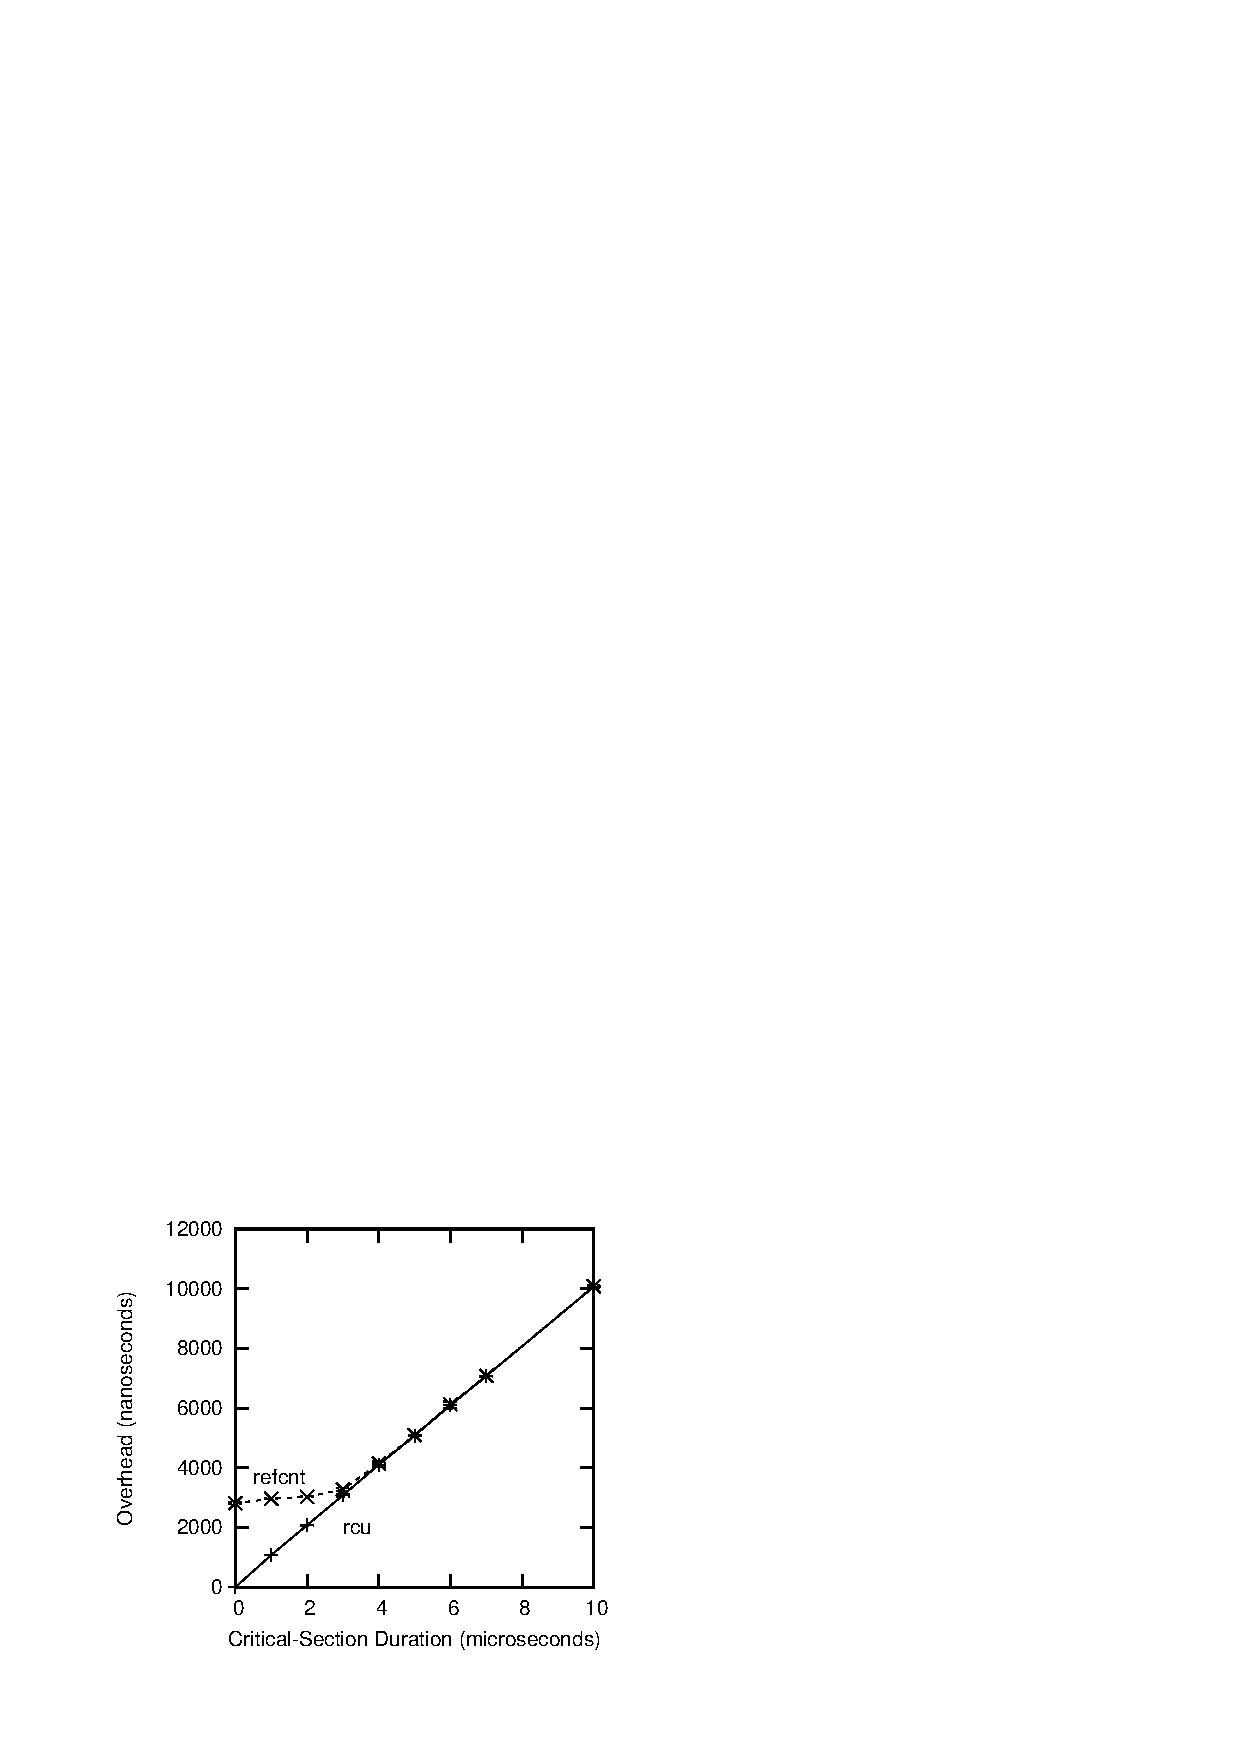
\includegraphics{defer/refRCUperfwtPREEMPT}}
\end{center}
\caption{Response Time of RCU vs. Reference Counting}
\label{fig:defer:Response Time of RCU vs. Reference Counting}
\end{figure}

And, as with reader-writer locking, the performance advantages
of RCU are most pronounced for short-duration critical sections, as shown
Figure~\ref{fig:defer:Response Time of RCU vs. Reference Counting}
for a 16-CPU system.
In addition, as with reader-writer locking, many system calls (and thus
any RCU read-side critical sections that they contain) complete in
a few microseconds.

However, the restrictions that go with RCU can be quite onerous.
For example, in many cases, the prohibition against sleeping while in an RCU
read-side critical section would defeat the entire purpose.
The next section looks at ways of addressing this problem, while also
reducing the complexity of traditional reference counting, at least in
some cases.

\subsubsection{RCU is a Bulk Reference-Counting Mechanism}
\label{sec:defer:RCU is a Bulk Reference-Counting Mechanism}

As noted in the preceding section,
traditional reference counters are usually associated with a specific
data structure, or perhaps a specific group of data structures.
However, maintaining a single global reference counter for a large
variety of data structures typically results in bouncing
the cache line containing the reference count.
Such cache-line bouncing can severely degrade performance.

In contrast, RCU's light-weight read-side primitives permit
extremely frequent read-side usage with negligible performance
degradation, permitting RCU to be used as a "bulk reference-counting"
mechanism with little or no performance penalty.
Situations where a reference must be held by a single task across a
section of code that blocks may be accommodated with
Sleepable RCU (SRCU)~\cite{PaulEMcKenney2006c}.
This fails to cover the not-uncommon situation where a reference is "passed"
from one task to another, for example, when a reference is acquired
when starting an I/O and released in the corresponding completion
interrupt handler.
(In principle, this could be handled by the SRCU implementation,
but in practice, it is not yet clear whether this is a good tradeoff.)

Of course, SRCU brings restrictions of its own, namely that the
return value from \url{srcu_read_lock()} be passed into the
corresponding \url{srcu_read_unlock()}, and that no SRCU primitives
be invoked from hardware irq handlers or from NMI/SMI handlers.
The jury is still out as to how much of a problem is presented by
these restrictions, and as to how they can best be handled.

\subsubsection{RCU is a Poor Man's Garbage Collector}
\label{sec:defer:RCU is a Poor Man's Garbage Collector}

A not-uncommon exclamation made by people first learning about
RCU is "RCU is sort of like a garbage collector!".
This exclamation has a large grain of truth, but it can also be
misleading.

Perhaps the best way to think of the relationship between RCU
and automatic garbage collectors (GCs) is that RCU resembles
a GC in that the \emph{timing} of collection is automatically
determined, but that RCU differs from a GC in that: (1) the programmer
must manually indicate when a given data structure is eligible
to be collected, and (2) the programmer must manually mark the
RCU read-side critical sections where references might legitimately
be held.

Despite these differences, the resemblance does go quite deep,
and has appeared in at least one theoretical analysis of RCU.
Furthermore, the first RCU-like mechanism I am aware of used
a garbage collector to handle the grace periods.
Nevertheless, a better way of thinking of RCU is described in the
following section.

\subsubsection{RCU is a Way of Providing Existence Guarantees}
\label{sec:defer:RCU is a Way of Providing Existence Guarantees}

Gamsa et al.~\cite{Gamsa99}
discuss existence guarantees and describe how a mechanism
resembling RCU can be used to provide these existence guarantees
(see section~5 on page 7 of the PDF), and
Section~\ref{sec:locking:Lock-Based Existence Guarantees}
discusses how to guarantee existence via locking, along with the
ensuing disadvantages of doing so.
The effect is that if any RCU-protected data element is accessed
within an RCU read-side critical section, that data element is
guaranteed to remain in existence for the duration of that RCU
read-side critical section.

\begin{figure}[tbp]
{ \scriptsize
\begin{verbatim}
  1 int delete(int key)
  2 {
  3   struct element *p;
  4   int b;
  5   5
  6   b = hashfunction(key);
  7   rcu_read_lock();
  8   p = rcu_dereference(hashtable[b]);
  9   if (p == NULL || p->key != key) {
 10     rcu_read_unlock();
 11     return 0;
 12   }
 13   spin_lock(&p->lock);
 14   if (hashtable[b] == p && p->key == key) {
 15     rcu_read_unlock();
 16     hashtable[b] = NULL;
 17     spin_unlock(&p->lock);
 18     synchronize_rcu();
 19     kfree(p);
 20     return 1;
 21   }
 22   spin_unlock(&p->lock);
 23   rcu_read_unlock();
 24   return 0;
 25 }
\end{verbatim}
}
\caption{Existence Guarantees Enable Per-Element Locking}
\label{fig:defer:Existence Guarantees Enable Per-Element Locking}
\end{figure}

Figure~\ref{fig:defer:Existence Guarantees Enable Per-Element Locking}
demonstrates how RCU-based existence guarantees can enable
per-element locking via a function that deletes an element from
a hash table.
Line~6 computes a hash function, and line~7 enters an RCU
read-side critical section.
If line~9 finds that the corresponding bucket of the hash table is
empty or that the element present is not the one we wish to delete,
then line~10 exits the RCU read-side critical section and line~11
indicates failure.

\QuickQuiz{}
	What if the element we need to delete is not the first element
	of the list on line~9 of
	Figure~\ref{fig:defer:Existence Guarantees Enable Per-Element Locking}?
\QuickQuizAnswer{
	As with
	Figure~\ref{fig:locking:Per-Element Locking Without Existence Guarantees},
	this is a very simple hash table with no chaining, so the only
	element in a given bucket is the first element.
	The reader is again invited to adapt this example to a hash table with
	full chaining.
} \QuickQuizEnd

Otherwise, line~13 acquires the update-side spinlock, and
line~14 then checks that the element is still the one that we want.
If so, line~15 leaves the RCU read-side critical section,
line~16 removes it from the table, line~17 releases
the lock, line~18 waits for all pre-existing RCU read-side critical
sections to complete, line~19 frees the newly removed element,
and line~20 indicates success.
If the element is no longer the one we want, line~22 releases
the lock, line~23 leaves the RCU read-side critical section,
and line~24 indicates failure to delete the specified key.

\QuickQuiz{}
	Why is it OK to exit the RCU read-side critical section on
	line~15 of
	Figure~\ref{fig:defer:Existence Guarantees Enable Per-Element Locking}
	before releasing the lock on line~17?
\QuickQuizAnswer{
	First, please note that the second check on line~14 is
	necessary because some other
	CPU might have removed this element while we were waiting
	to acquire the lock.
	However, the fact that we were in an RCU read-side critical section
	while acquiring the lock guarantees that this element could not
	possibly have been re-allocated and re-inserted into this
	hash table.
	Furthermore, once we acquire the lock, the lock itself guarantees
	the element's existence, so we no longer need to be in an
	RCU read-side critical section.

	The question as to whether it is necessary to re-check the
	element's key is left as an exercise to the reader.
} \QuickQuizEnd

\QuickQuiz{}
	Why not exit the RCU read-side critical section on
	line~23 of
	Figure~\ref{fig:defer:Existence Guarantees Enable Per-Element Locking}
	before releasing the lock on line~22?
\QuickQuizAnswer{
	Suppose we reverse the order of these two lines.
	Then this code is vulnerable to the following sequence of
	events:
	\begin{enumerate}
	\item	CPU~0 invokes \url{delete()}, and finds the element
		to be deleted, executing through line~15.
		It has not yet actually deleted the element, but
		is about to do so.
	\item	CPU~1 concurrently invokes \url{delete()}, attempting
		to delete this same element.
		However, CPU~0 still holds the lock, so CPU~1 waits
		for it at line~13.
	\item	CPU~0 executes lines~16 and 17, and blocks at
		line~18 waiting for CPU~1 to exit its RCU read-side
		critical section.
	\item	CPU~1 now acquires the lock, but the test on line~14
		fails because CPU~0 has already removed the element.
		CPU~1 now executes line~22 (which we switched with line~23
		for the purposes of this Quick Quiz)
		and exits its RCU read-side critical section.
	\item	CPU~0 can now return from \url{synchronize_rcu()},
		and thus executes line~19, sending the element to
		the freelist.
	\item	CPU~1 now attempts to release a lock for an element
		that has been freed, and, worse yet, possibly
		reallocated as some other type of data structure.
		This is a fatal memory-corruption error.
	\end{enumerate}
} \QuickQuizEnd

Alert readers will recognize this as only a slight variation on
the original "RCU is a way of waiting for things to finish" theme,
which is addressed in
Section~\ref{sec:deferRCU is a Way of Waiting for Things to Finish}.
They might also note the deadlock-immunity advantages over the lock-based
existence guarantees discussed in
Section~\ref{sec:locking:Lock-Based Existence Guarantees}.

\subsubsection{RCU is a Way of Providing Type-Safe Memory}
\label{sec:deferRCU is a Way of Providing Type-Safe Memory}

A number of lockless algorithms do not require that a given data
element keep the same identity through a given RCU read-side critical
section referencing it---but only if that data element retains the
same type.
In other words, these lockless algorithms can tolerate a given data
element being freed and reallocated as the same type of structure
while they are referencing it, but must prohibit a change in type.
This guarantee, called ``type-safe memory'' in
academic literature~\cite{Cheriton96a},
is weaker than the existence guarantees in the
previous section, and is therefore quite a bit harder to work with.
Type-safe memory algorithms in the Linux kernel make use of slab caches,
specially marking these caches with \url{SLAB_DESTROY_BY_RCU}
so that RCU is used when returning a freed-up
slab to system memory.
This use of RCU guarantees that any in-use element of
such a slab will remain in that slab, thus retaining its type,
for the duration of any pre-existing RCU read-side critical sections.

\QuickQuiz{}
	But what if there is an arbitrarily long series of RCU
	read-side critical sections in multiple threads, so that at
	any point in time there is at least one thread in the system
	executing in an RCU read-side critical section?
	Wouldn't that prevent any data from a \url{SLAB_DESTROY_BY_RCU}
	slab ever being returned to the system, possibly resulting
	in OOM events?
\QuickQuizAnswer{
	There could certainly be an arbitrarily long period of time
	during which at least one thread is always in an RCU read-side
	critical section.
	However, the key words in the description in
	Section~\ref{sec:deferRCU is a Way of Providing Type-Safe Memory}
	are ``in-use'' and ``pre-existing''.
	Keep in mind that a given RCU read-side critical section is
	conceptually only permitted to gain references to data elements
	that were in use at the beginning of that critical section.
	Furthermore, remember that a slab cannot be returned to the
	system until all of its data elements have been freed, in fact,
	the RCU grace period cannot start until after they have all been
	freed.

	Therefore, the slab cache need only wait for those RCU read-side
	critical sections that started before the freeing of the last element
	of the slab.
	This in turn means that any RCU grace period that begins after
	the freeing of the last element will do---the slab may be returned
	to the system after that grace period ends.
} \QuickQuizEnd

These algorithms typically use a validation step that checks to make
sure that the newly referenced data structure really is the one that
was requested~\cite[Section 2.5]{LaninShasha1986TSM}.
These validation checks require that portions of the data structure
remain untouched by the free-reallocate process.
Such validation checks are usually very hard to get right, and can
hide subtle and difficult bugs.

Therefore, although type-safety-based lockless algorithms can be extremely
helpful in a very few difficult situations, you should instead use existence
guarantees where possible.
Simpler is after all almost always better!

\subsubsection{RCU is a Way of Waiting for Things to Finish}
\label{sec:deferRCU is a Way of Waiting for Things to Finish}

As noted in Section~\ref{sec:defer:RCU Fundamentals}
an important component
of RCU is a way of waiting for RCU readers to finish.
One of
RCU's great strengths is that it allows you to wait for each of
thousands of different things to finish without having to explicitly
track each and every one of them, and without having to worry about
the performance degradation, scalability limitations, complex deadlock
scenarios, and memory-leak hazards that are inherent in schemes that
use explicit tracking.

In this section, we will show how \url{synchronize_sched()}'s
read-side counterparts (which include anything that disables preemption,
along with hardware operations and
primitives that disable irq) permit you to implement interactions with
non-maskable interrupt (NMI)
handlers that would be quite difficult if using locking.
This approach has been called "Pure RCU"~\cite{PaulEdwardMcKenneyPhD},
and it is used in a number of places in the Linux kernel.

The basic form of such "Pure RCU" designs is as follows:

\begin{enumerate}
\item	Make a change, for example, to the way that the OS reacts to an NMI.
\item	Wait for all pre-existing read-side critical sections to
	completely finish (for example, by using the
	\url{synchronize_sched()} primitive).
	The key observation here is that subsequent RCU read-side critical
	sections are guaranteed to see whatever change was made.
\item	Clean up, for example, return status indicating that the
	change was successfully made.
\end{enumerate}

The remainder of this section presents example code adapted from
the Linux kernel.
In this example, the \url{timer_stop} function uses
\url{synchronize_sched()} to ensure that all in-flight NMI
notifications have completed before freeing the associated resources.
A simplified version of this code is shown
Figure~\ref{fig:defer:Using RCU to Wait for NMIs to Finish}.

\begin{figure}[tbp]
{ \scriptsize
\begin{verbatim}
  1 struct profile_buffer {
  2   long size;
  3   atomic_t entry[0];
  4 };
  5 static struct profile_buffer *buf = NULL;
  6
  7 void nmi_profile(unsigned long pcvalue)
  8 {
  9   struct profile_buffer *p = rcu_dereference(buf);
 10
 11   if (p == NULL)
 12     return;
 13   if (pcvalue >= p->size)
 14     return;
 15   atomic_inc(\&p->entry[pcvalue]);
 16 }
 17
 18 void nmi_stop(void)
 19 {
 20   struct profile_buffer *p = buf;
 21
 22   if (p == NULL)
 23     return;
 24   rcu_assign_pointer(buf, NULL);
 25   synchronize_sched();
 26   kfree(p);
 27 }
\end{verbatim}
}
\caption{Using RCU to Wait for NMIs to Finish}
\label{fig:defer:Using RCU to Wait for NMIs to Finish}
\end{figure}

Lines~1-4 define a \url{profile_buffer} structure, containing a
size and an indefinite array of entries.
Line~5 defines a pointer to a profile buffer, which is
presumably initialized elsewhere to point to a dynamically allocated
region of memory.

Lines~7-16 define the \url{nmi_profile()} function,
which is called from within an NMI handler.
As such, it cannot be preempted, nor can it be interrupted by a normal
irq handler, however, it is still subject to delays due to cache misses,
ECC errors, and cycle stealing by other hardware threads within the same
core.
Line~9 gets a local pointer to the profile buffer using the
\url{rcu_dereference()} primitive to ensure memory ordering on
DEC Alpha, and
lines~11 and 12 exit from this function if there is no
profile buffer currently allocated, while lines~13 and 14
exit from this function if the \url{pcvalue} argument
is out of range.
Otherwise, line~15 increments the profile-buffer entry indexed
by the \url{pcvalue} argument.
Note that storing the size with the buffer guarantees that the
range check matches the buffer, even if a large buffer is suddenly
replaced by a smaller one.

Lines~18-27 define the \url{nmi_stop()} function,
where the caller is responsible for mutual exclusion (for example,
holding the correct lock).
Line~20 fetches a pointer to the profile buffer, and
lines~22 and 23 exit the function if there is no buffer.
Otherwise, line~24 NULLs out the profile-buffer pointer
(using the \url{rcu_assign_pointer()} primitive to maintain
memory ordering on weakly ordered machines),
and line~25 waits for an RCU Sched grace period to elapse,
in particular, waiting for all non-preemptible regions of code,
including NMI handlers, to complete.
Once execution continues at line~26, we are guaranteed that
any instance of \url{nmi_profile()} that obtained a
pointer to the old buffer has returned.
It is therefore safe to free the buffer, in this case using the
\url{kfree()} primitive.

\QuickQuiz{}
	Suppose that the \url{nmi_profile()} function was preemptible.
	What would need to change to make this example work correctly?
\QuickQuizAnswer{
	One approach would be to use
	\url{rcu_read_lock()} and \url{rcu_read_unlock()}
	in \url{nmi_profile()}, and to replace the
	\url{synchronize_sched()} with \url{synchronize_rcu()},
	perhaps as shown in
	Figure~\ref{fig:defer:Using RCU to Wait for Mythical Preemptible NMIs to Finish}.

\begin{figure}[tbp]
{ \tt \scriptsize
\begin{verbatim}
  1 struct profile_buffer {
  2   long size;
  3   atomic_t entry[0];
  4 };
  5 static struct profile_buffer *buf = NULL;
  6
  7 void nmi_profile(unsigned long pcvalue)
  8 {
  9   struct profile_buffer *p;
 10
 11   rcu_read_lock();
 12   p = rcu_dereference(buf);
 13   if (p == NULL) {
 14     rcu_read_unlock();
 15     return;
 16   }
 17   if (pcvalue >= p->size) {
 18     rcu_read_unlock();
 19     return;
 20   }
 21   atomic_inc(&p->entry[pcvalue]);
 22   rcu_read_unlock();
 23 }
 24
 25 void nmi_stop(void)
 26 {
 27   struct profile_buffer *p = buf;
 28
 29   if (p == NULL)
 30     return;
 31   rcu_assign_pointer(buf, NULL);
 32   synchronize_rcu();
 33   kfree(p);
 34 }
\end{verbatim}
}
\caption{Using RCU to Wait for Mythical Preemptible NMIs to Finish}
\label{fig:defer:Using RCU to Wait for Mythical Preemptible NMIs to Finish}
\end{figure}

} \QuickQuizEnd

In short, RCU makes it easy to dynamically switch among profile
buffers (you just \emph{try} doing this efficiently with atomic
operations, or at all with locking!).
However, RCU is normally used at a higher level of abstraction, as
was shown in the previous sections.

\subsubsection{RCU Usage Summary}
\label{sec:defer:RCU Usage Summary}

At its core, RCU is nothing more nor less than an API that provides:

\begin{enumerate}
\item	a publish-subscribe mechanism for adding new data,
\item	a way of waiting for pre-existing RCU readers to finish, and
\item	a discipline of maintaining multiple versions to permit change
	without harming or unduly delaying concurrent RCU readers.
\end{enumerate}

That said, it is possible to build higher-level constructs
on top of RCU, including the reader-writer-locking, reference-counting,
and existence-guarantee constructs listed in the earlier sections.
Furthermore, I have no doubt that the Linux community will continue to
find interesting new uses for RCU,
as well as for any of a number of other synchronization primitives.

% <h3>Acknowledgements</h3> @@@
%
% We are all indebted to Andy Whitcroft, Jon Walpole, and Gautham Shenoy,
% whose review of an early draft of this document greatly improved it.
% I owe thanks to the members of the Relativistic Programming project
% and to members of PNW TEC for many valuable discussions.
% I am grateful to Dan Frye for his support of this effort.
